\section{Machine Learning}
%\todo{Write machine learning intro}
\acf{ml} is the discipline of defining a statistical or mathematical models based on data. These \ac{ml} models are either trained in a supervised or unsupervised fashion, which usually results in them learning a decision boundary, or a representation or structure of the data respectively. Historically, \ac{ml} has been an interest in geoscience but has not gained momentum due to sparse data, computational capability, and availability of algorithms. Geoscience data was often not available and still is often not available with a reliable ground truth. However, particularly \acp{nn} have found broad interest in geophysical applications, Bayesian methods are often used in inversion schemes and recent software developments have changed the research entirely.

% Development of Deep Learning
Recently, the subfield \ac{dl} has reignited interest in the wider field of \ac{ml} by outperforming rule-based algorithms on computer vision tasks, such as image classification and segmentation \citep{Bishop2016-mj}. These developments have propelled developments in other non-related fields such as biology \citep{Ching2018-hg}, chemistry \citep{Schutt2017-sh}, medicine \citep{Shen2017-nt} and pharmacology \citep{Kadurin2017-oq}. \ac{dl} utilizes many-layered artificial \ac{nn} to approximate an objective function. In recent years the open source movement, democratization of access to computing power and developments in the field of \ac{dl} have rekindled interest in applications of \ac{ml} to geoscience. The availability of free open source libraries such as skikit-learn \citep{scikit-learn} has made \ac{ml} methods and several tools for the application of rigorous statistical evaluation of experiments without explicit expert knowledge widely available. Furthermore, Tensorflow \citep{tensorflow}, PyTorch \citep{pytorch}, and Keras \citep{keras} have made \acp{nn} easily accessible and provide experimentation capabilities to transfer recent developments in \ac{ml} research to other scientific fields. 


Algorithms and methods in \ac{ml} can be organized in different ways. Two ways to categorize algorithms are based on the training or based on the learned distribution. In training, these algorithms can be categorized into supervised and unsupervised methods, where supervised methods learn the functional mapping from $x$, being the data, to $y$, being the ground truth or label for the data. When the ground truth is not known, unsupervised methods can be applied to determine structures and relationships within the data. Semi-supervised, and weakly supervised try to propagate partial labels to similarly distributed data and then learn the supervised mapping f(x) = y. Alternatively, \ac{ml} algorithms can be categorized into generative methods that learn the joint probability distribution or discriminative methods that learn a decision boundary to optimally separate data. Additionally, methods can be distinguished by application. Assigning labels to data is called classification. The general, continuous application to map data from the input to the output domain is called regression. Finding relationships and agglomerations of data is called clustering. Most algorithms can be applied to several of these categories, such as support vector machines that can function as classifier and regressor. 

Applications in \ac{ml} are quickly evolving and many are improved by mathematical insights, engineering features and increased availability of data. This thesis focuses on the application of \acp{nn}, which come in different implementation details and particularly \ac{nn} architectures are often re-implemented with slight differences that deviate from the original published architecture. Particularly in \ac{nn} we have to focus on the most practical building blocks, to be able to give a comprehensive overview.

\subsection{History of Machine Learning}

\begin{figure}[!ht]
    \centering
    \hspace*{-1.5cm}
    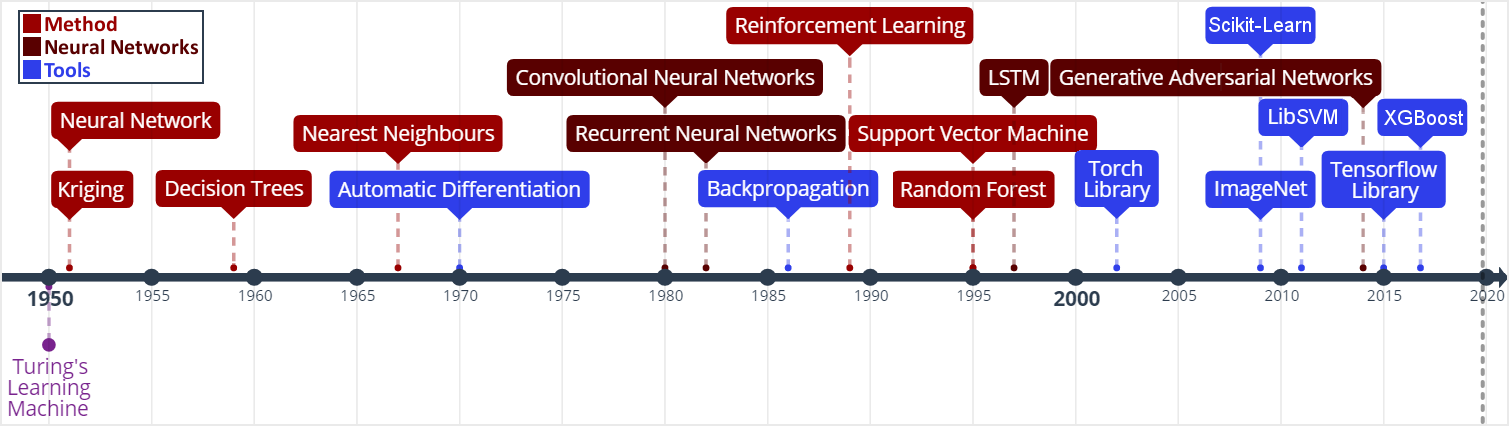
\includegraphics[width=1.15\textwidth]{figures/ML-Timeline.png}
    \caption{Selection of notable milestones in machine learning}
    \label{fig:mltimeline}
\end{figure}

Creativity, learning, and intelligence with regard to computers have been discussed as early as of the first programmer Ada Lovelace \citep{taylor1843scientific}.

\begin{quote}
    "The Anlytical Engine has no pretensions whatever to \textit{originate} any thing. It can do whatever we \textit{know how to order it} to perform. It can \textit{follow} analysis; but it has no power of \textit{anticipating} any analytical relations or truths. Its province is to assist us in making \textit{available} what we are already acquainted with. This it is calculated too effect primarily and chiefly of course, through its executive faculties; but it is likely to exert an \textit{indirect} and reciprocal influence on science itself in another manner." -- Note G, Page 689, Ada A. Lovelace. \citep{taylor1843scientific}; Emphasis taken from source text.
\end{quote}

This notion was challenged by Alan Turing \citep{turing1950} who proposed the "Learning Machine", which specifically predict genetic algorithms, a metaheuristic that finds application in optimization and search problems. Evolutionary computing and genetic algorithms specifically can perform some machine learning tasks \citep{Goldberg1988-ch}. This is generally considered the commencement of \ac{ai} and \ac{ml}, however, they rely heavily on earlier developments in statistics such as the Bayesian theorem \citep{bayes1763lii} and Markov processes \citep{markov1906rasprostranenie,markov1971extension}. The first method, we include on the timeline in \cref{fig:mltimeline} is "kriging" \citep{Krige1951}, which is based on Gaussian Processes, these form an important category of non-parametric machine learning these days. Gaussian processes are often also attributed to work of \citet{kolmogorov1939interpolation} on time series. Another method was developed to mimic the human brain, namely \acfp{nn}. The construction of the first \ac{nn} machine by Minsky \citep{russelnorvig} was soon followed by the "Perceptron", a binary decision boundary learner \citep{rosenblatt1958perceptron}. The decision is made according to

\begin{equation}
\begin{array}{ll}
    o_{j} & = \sigma \left(\sum_i w_{ij} x_{i} + b\right)\\
    & = \begin{cases}1&\sum_i w_{ij} x_{i} + b > 0 \\ 0 &\text{otherwise}   \end{cases}
\end{array}
\end{equation}
which describes a linear system of the input data $x$, the weights $w$ and bias $b$ and a binary activation funtion $\sigma$. The linear system is still used in modern neurons, however, the activation $\sigma$ is usually a Rectifier function. Shortly after, \citet{belson1959matching} describe the first \acf{dt}, which learns hierarchical decision systems. The next method, \ac{knn} search, was introduced by \citet{cover1967nearest} to solve the traveling salesman problem. Two decades later Q-learning \citep{watkins1989learning} introduces a method to reinforcement learning that is still used to this day. The final two methods in the timeline were introduced in 1995. \acfp{rf} \citep{ho1995random} introduce ensemble learning of weak learning \acfp{dt}. \acf{svm} \citep{cortes1995support} introduce a strong learner that aims to maximize the margin between classes.

These methods have been improved upon over the decades. Specific milestones that accelerated further developments in \ac{nn} are automatic differentiation \citep{linnainmaa1970representation} and consequently applying this to backpropagate errors in \acp{dnn} \citep{rumelhart1988learning}. Backpropagation itself as a concept existed earlier \citep{kelley1960gradient, bryson1961gradient}, followed by a simplification by using the chain rule \citep{dreyfus1962numerical}. These enable effective implementation of \acp{nn} today. Moreover, open sourcing the Torch library \citep{collobert2002torch} made and assembling the ImageNet database \citep{deng2009imagenet} has accelerated developments in computer vision and enabled modern developments in deep learning. In the same year of 2009 the library Scikit-Learn \citep{scikit-learn} was established, which introduced a common open source \ac{api} \citep{sklearn_api} for a diverse and growing set of shallow machine learning models (e.g. \acp{svm}, \acp{rf}, \acp{knn}, shallow \acp{nn}). Scikit-learn has had a profound impact on machine learning applications across the sciences and the API is modelled in other open source libraries. \citet{libsvm} introduced a widely used implementation for \acf{svm}, which is also used in Scikit-Learn. Recently, the Tensorflow library \citep{tensorflow} was introduced for open source deep learning models, with some different design choices than Pytorch. In this open environment fueled by competitions (e.g. ImageNet \citep{ILSVRCanalysis_ICCV2013}, Netflix Prize \citep{bennett2007netflix}, Kaggle \citep{goodfellow2013challenges}) XGBoost \citep{xgboost}, a library for extreme gradient tree boosting was developed.

Recent developments in deep learning are based in \acfp{nn}, hence, we highlight some key developments in \cref{fig:mltimeline}. \acfp{cnn} are essential in the modern computational vision systems, they were inspired by the concept of Neocognitron \citep{fukushima1980neocognitron, lecun2015deep}. In the same decade \acfp{rnn} were introduced implemented as Hopfield Networks \citep{hopfield1982neural}. While Hopfield networks are not a general \ac{rnn}, they provide content-adressable memory with the internal state memory. \citet{hochreiter1997long} implement the \acf{lstm}, which contain internal states (i.e. memory) that can process temporal sequences, still used and performing to the state-of-the-art in sequence analysis and \ac{nlp} to this day. Recently, \acf{gan} \citep{goodfellow2014generative} introduced a system of \acp{nn} that can create new samples from a distribution. The \ac{gan} consists of two \acp{nn}, a generator and a discriminator, which generate samples from a noise distribution and judge the validity of the sample respectively. We discuss \acp{nn} in more detail in \cref{section:nn}

\subsection{\acfp{nn}}
\label{section:nn}
\acf{nn} as a class of \ac{ml} algorithms are very diverse and versatile. \acp{nn} have persisted for decades and their nomenclature has changed in this time. \acp{nn} were long called \ac{ann}, which has changed to simply \ac{nn}, usually prepended with the class of \acl{nn}, namely  \acf{rnn}, \acf{cnn}, \acf{dnn}, which I will discuss in more detail.

\begin{figure}
    \centering
    \includesvg[width=\textwidth,height=5cm]{{figures/Single-Layer_Neural_Network}}
    \caption{Basic \ac{nn} with three inputs that are densely connected to three output neurons by weights}
    \label{fig:simpleneuralnetwork}
\end{figure}

\acfp{nn} can be approached from several theoretical bases. Mathematically, \acp{nn} are directed acyclical graphs with edges and nodes. In neural computation, these are generally referred to as weights and nodes or neurons. In \cref{fig:simpleneuralnetwork}, we present a simple densely connected \ac{mlp} with three inputs and three outputs. This configuration is equivalent to a linear regression model. The inputs are distributed across the nodes, and each weight is multiplied with a weight inherent to that graph edge. During the training of this machine learning model, these weights get adjusted to obtain a generalizable result. Each node sums the contributions of these weights and possibly a bias, which is trainable but does not take input data. This amounts to each node performing

\begin{equation}
    a_{j} = \sigma \left(\sum_i w_{ij} x_{i} + b\right),
\end{equation}
with $a$ signifying the activation at a node, $i,j$ being the index of the source and target node respectively, $w$ being the trainable weight, and $b$ being the trainable bias, and $\sigma$ representing an activation function. Activation functions are an active topic of research, but the generally perform a non-linear transformation of the activation at the node.

\begin{figure}
    \centering
    \subbottom[Linear activation]{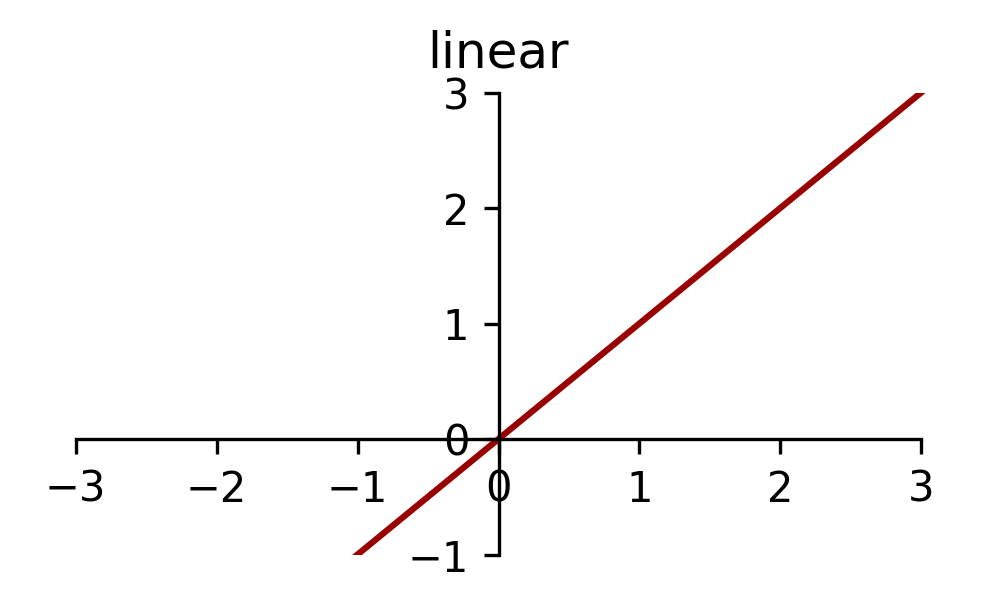
\includegraphics[width=.35\textwidth]{figures/activations/act_linear.png}\label{fig:act_lin}}%
    \subbottom[Sigmoid activation]{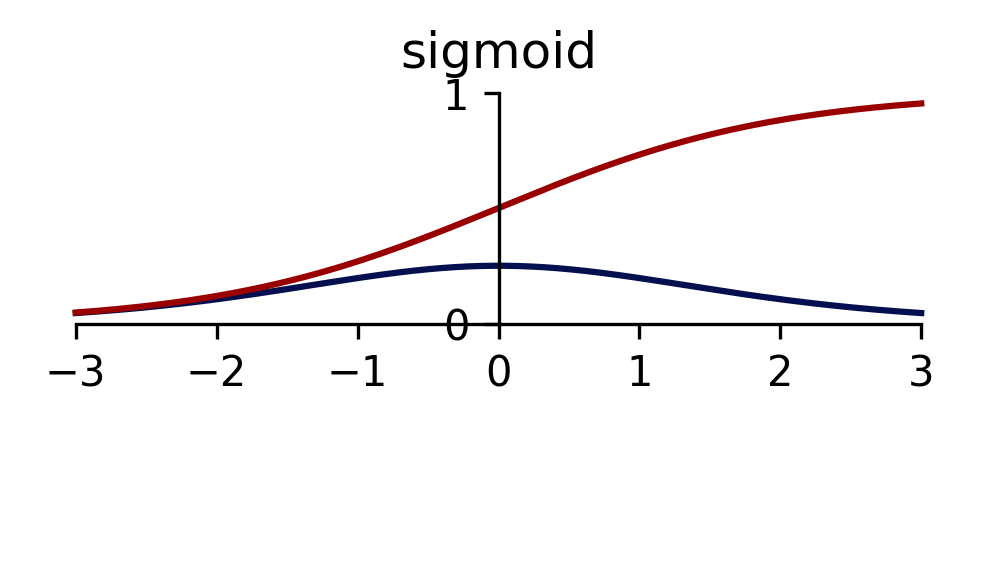
\includegraphics[width=.35\textwidth]{figures/activations/act_sigmoid.png}\label{fig:act_sig}}%
    \subbottom[Tanh activation]{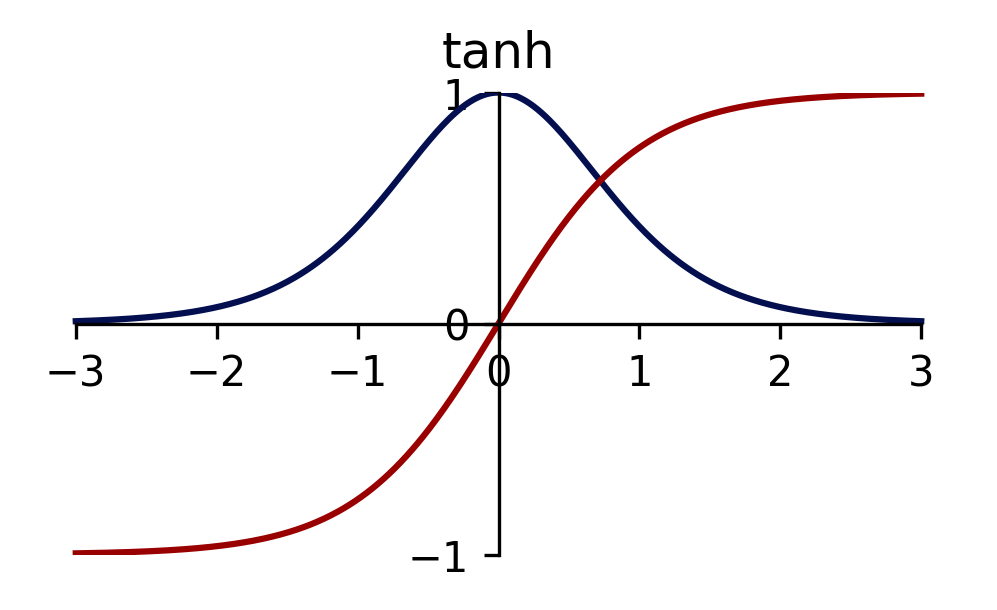
\includegraphics[width=.35\textwidth]{figures/activations/act_tanh.png}\label{fig:act_tanh}}%
    \\
    \subbottom[\ac{relu} activation]{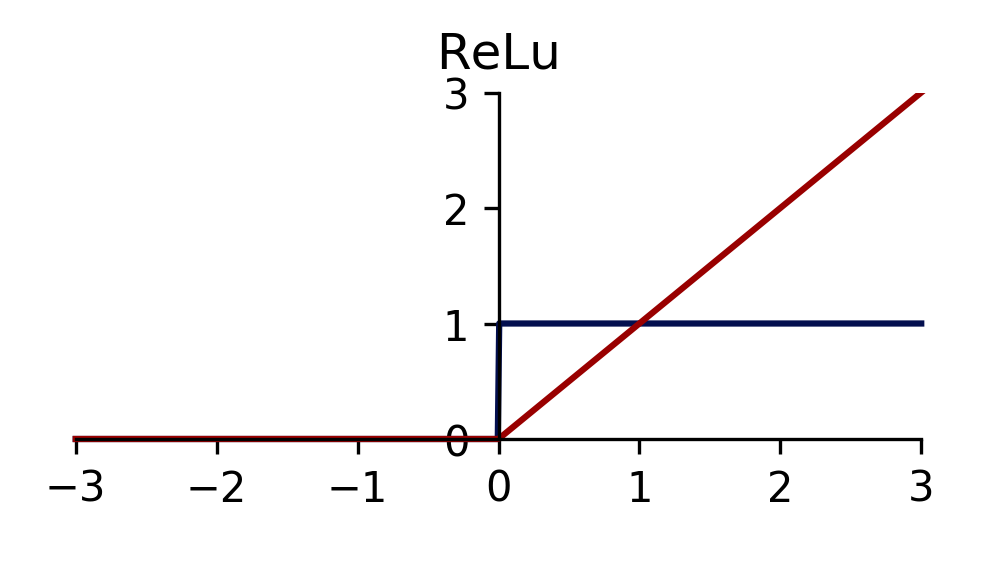
\includegraphics[width=.35\textwidth]{figures/activations/act_relu.png}\label{fig:act_relu}}%
    \subbottom[\ac{prelu} activation ($\alpha=.5$)]{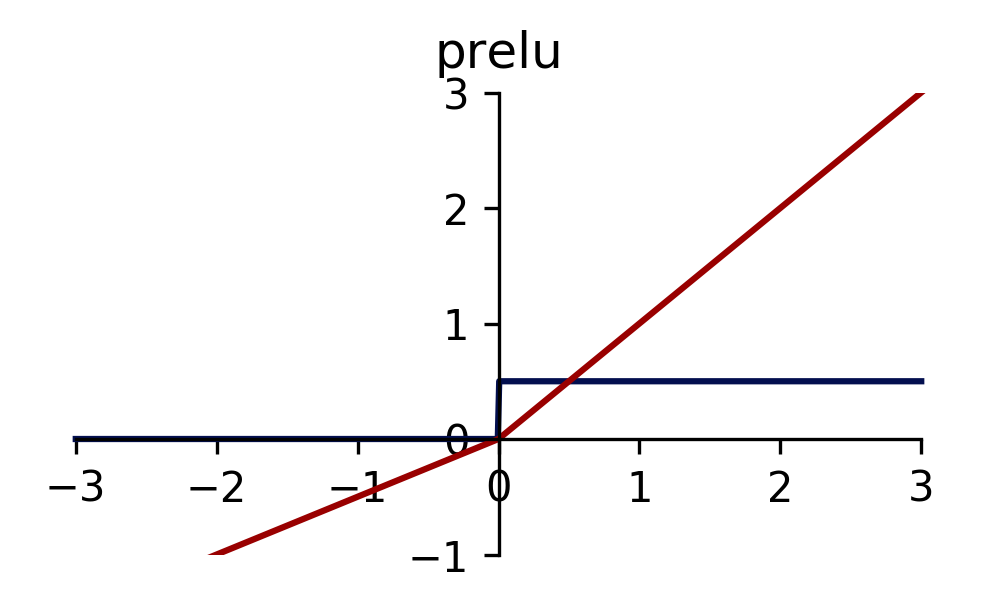
\includegraphics[width=.35\textwidth]{figures/activations/act_prelu.png}\label{fig:act_prelu}}%
    \subbottom[\ac{elu} activation ($\alpha=1$)]{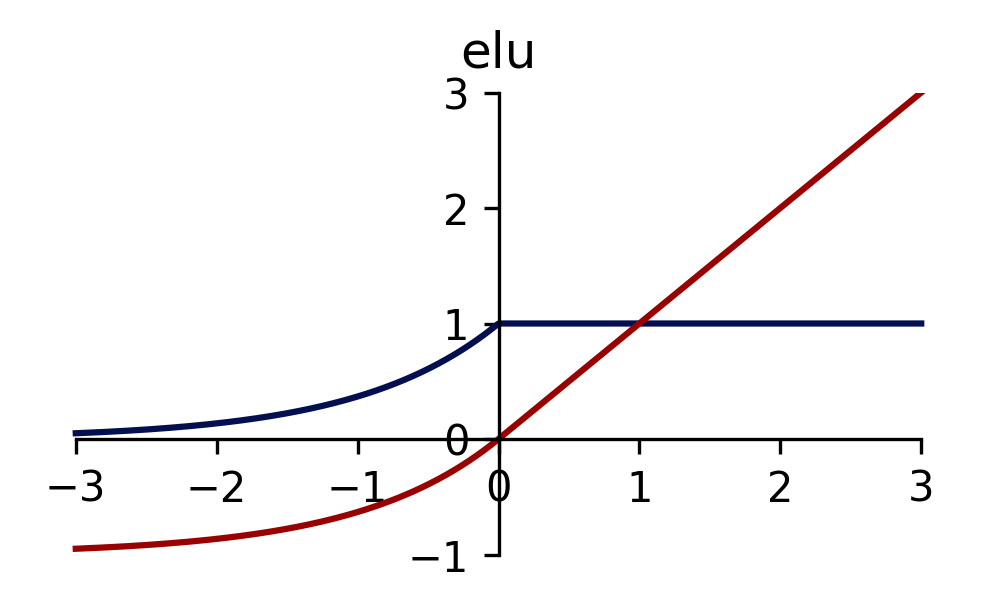
\includegraphics[width=.35\textwidth]{figures/activations/act_elu.png}\label{fig:act_elu}}
    \caption{Common Activation functions (red) and derivatives (blue). The linear activation does not modify the data. The sigmoid and tanh functions are mainly used to limit output activations to a range of values. The \ac{relu}, \ac{prelu} and \ac{elu} activations are different iterations of rectifiers that are used in \aclp{dnn}}
    \label{fig:activations}
\end{figure}

In \cref{fig:activations} I present common activation functions used in \acp{nn}. The activation functions introduce non-linearities into the network to transform the linearly scaled input to arbitrary non-linear outputs. The mathematical function in \cref{fig:act_sig} and \cref{fig:act_tanh} are used less, because of the vanishing gradient problem \citep{hochreiter1991untersuchungen}. These occur in the extrema of both functions, where the function saturates and the gradient is close to zero for large values of x. Rectifiers presented in \cref{fig:act_relu,fig:act_prelu,fig:act_elu} circumvent this problem by one-sided saturation. 

\paragraph{Training the Model} 
Before training, each weight and bias is assigned an initial number that is drawn from a distribution appropriate to the network architecture and data \citep{lecun2012efficient, glorot2010understanding, he2015delving}. These strategies collectively initialize weights in a pseudo-random way within limits. The data is then passed through the network, which calculates a result. This result is then compared to the ground truth, using a loss function (e.g. \ac{mae}, \ac{mse}). The resulting error $\Delta t$ is then used to correct the weights and biases in the network, calculating the correction per weight $\Delta w_{ij}$ recursively (for many-layered networks).
\begin{equation}
    \Delta w_{ij}= -\eta \dfrac{\partial E}{\partial w_{ij}} = -\eta \delta_{j} a_{i},
\end{equation}
with $\eta$ being the learning rate and $\delta$ being
\begin{equation}
    \delta_{j}=\begin{cases}
\sigma'( \text{net}_{j} ) \Delta t              & \text{if } j \text{ is output node,}\\
\sigma'( \text{net}_{j} ) \sum_{j-1} \delta_{j-1} w_{j(j-1)} & \text{if } j \text{ is hidden node.}
\end{cases}
\end{equation}
Therefore, hidden nodes are reliant on the result $\delta_{j-1}$ of the node at index $j-1$ \citep{deeplearningbook}. The training of the model can be done on a per-sample basis, which is \ac{sgd} or in the case of noisy inputs, the mean error of several samples can be calculated to perform mini-batch gradient descent. Iteration over forward and backward passes adjusts the weights to predict the correct result. 

Modern deep \acp{nn} are trained on \acp{gpu} that are optimized for matrix multiplications instead of \acp{cpu} that are magnitudes slower. However, more recently task-specific hardware such as \acp{fgpa} and \acp{tpu}, which work closely with the \ac{tf} library are being developed and made available in cloud infrastructures.

The optimization of the backpropagation is performed using \ac{sgd} or other gradient-based optimizers such as the Adam optimizer \citep{kingma2014adam}. However, during training of the \ac{nn}, it is important to ensure that the network learns a general relationship instead of memorizing the input data. This memorization is called overtraining, or overfitting. Overfitting can be avoided by regularizations like weight decay \citep{krogh1992simple} and Nesterov momentum \citep{pmlr-v28-sutskever13}, which modify the optimization loop. Alternatively, methods like Dropout \citep{hinton2012improving} and \ac{bn} \citep{ioffe2015batch} modify the network at training time. Moreover, a diverse training set and train-val-test split help avoid overfitting and ensure generalization of the trained model.

The train-val-test split separates the data into three parts. The training and validation set are available during training and hyperparameter tuning, the test set, however, should only be used once to ensure generalization of the model. The train test is used during the optimization loop, the actual training of the model, with the validation set ensuring generalization of the model to unseen data within the loop. In and of itself, the train and validation data would be sufficient, if no other changes to the model were made based on the results of the validation data. Since hyperparameter tuning and model selection are a common procedure today, these present an implicit source of information leakage from the validation set into the data. The hyperparameter tuning will often pose an optimization loop in itself that optimizes based on the results on the "unseen" validation set, essentially implicitly fitting the model to the validation data, therefore, a separate test set is necessary to ensure true generalization.


\subsubsection{Feed Forward Networks}
Feed forward \acfp{nn} or \acp{mlp} are the simplest for of \ac{nn}. In its simplest form it uses a set of linear equations to approximate a function. The network can be described as a graph with edges and nodes. In the neural information community the nodes are often named neurons. These neurons are arranged into layers in \cref{fig:feedneuralnetwork}. The first layer in a \ac{nn} is the input layer with a number of nodes corresponding to the number of input data points. The input nodes are connected to the next layer by the graph's edge. The next node can be the output layer. The weights between subsequent are floating point numbers that scale each input point and determine the value at the output nodes.

\begin{figure}
    \centering
    \includesvg[width=\textwidth,height=5cm]{{figures/Multi-Layer_Neural_Network-Vector}}
    \caption{Feed forward \ac{nn} with three input neurons that are connected to a single hidden layer with three neurons. The hidden layer is densely connected to two output neurons}
    \label{fig:feedneuralnetwork}
\end{figure}

\acp{nn} gain their powerful learning capabilities from adding layers (see \cref{fig:feedneuralnetwork}) in between the input and output node and applying a non-linear activation function. Non-linear activations scale the input from the edge at each neuron. Historically, these have been straight-forward mathematical functions such as $tanh()$ and $sig()$ (cf. \cref{fig:activations}). These suffer from some short-comings that were overcome to leverage multi-layered \acfp{dnn}.

\subsubsection{\acfp{dnn}}
\label{section:dnn}
Improvements in computational power made it possible to train many-layered \acp{nn} (see \cref{fig:deepneuralnetwork}). These \acfp{dnn} are at the core of recent developments in \acf{dl}, leading to the re-implementation of many algorithms into openly available libraries, which has led to further innovative uses of these building blocks. These networks leverage the combinatorial power of \ac{nn} layers. In deep \acp{nn} gradient propagation led to exploding or vanishing gradients before. New non-saturating activation functions lead to stabilization of training \ac{dnn} (cf. \cref{fig:activations}).

\begin{figure}
    \centering
    \includesvg[width=\textwidth,height=5cm]{{figures/Deep-Multi-Layer_Neural_Network-Vector}}
    \caption{Deep Feed forward \ac{nn} with two hidden layers with three neurons each, densely connected to three inputs and two output neurons. Deep networks are \acp{nn} that contain more than one hidden layer}
    \label{fig:deepneuralnetwork}
\end{figure}

\subsubsection{\acfp{som}}
\acf{som}, also named Kohonen-networks \citep{kohonen1982self} are a special case of networks that do not modify the flow of data from the input to the output nodes. They treat each data point as a node and adjust the weights between each node in on a similarity metric. These tend to perform well on spatially correlated data and find good adoption in geoscience.

\subsubsection{Recurrent Networks}
A special configuration of \ac{nn} is the \acf{rnn}. These networks use edges that feed back into the network. \acp{rnn} are used in two applications in \ac{ml}. They can preserve hidden states, which gives them temporal context sensitivity. Application two is time series analysis similar to feed-forward \acp{nn}, where the input is a time step that can be analyzed within the context of surrounding time steps. These \ac{rnn} represent cyclic directed graphs of computation, as opposed to the other types of \ac{nn} we discuss, which are acyclic directed graphs. 
In \cref{fig:recurrentneuralnetwork} we show the changes of a simple \ac{rnn} graph compared to a feed forward \ac{nn} in \cref{fig:feedneuralnetwork}. The \ac{rnn} loops back into itself, which is often regarded as the internal state or feedback. This internal state enables content addressable memory and good performance on sequential data such as time series and language.

\begin{figure}
    \centering
    \includesvg[width=\textwidth,height=5cm]{{figures/Recurrent-Layer_Neural_Network-Vector-Blank}}
    \caption{Recurrent \ac{nn} that connects two input neurons to two recurrent neurons. These recurrent neurons feed back into themselves, which signifies the state of the neuron. \ac{rnn} neurons are more complicated internally than the neurons in \acp{cnn} accomodating the state memory}
    \label{fig:recurrentneuralnetwork}
\end{figure}

\paragraph{Hopfield Networks} are one type of recurrent networks that model the human memory. Hopfield networks and their subclasses can be used for pattern recognition. They are guaranteed to find a pattern, however, they are known to converge to local minima. Boltzman machines are configured like Hopfield networks, in contrast to deterministic Hopfield networks, their response to an input is stochastic. Boltzman machines draw from a joint distribution, making them a generative model.

\paragraph{\acf{lstm}} is a type of \ac{rnn} that models memory. Details differ in implementations of \acf{lstm}, however the main criteria are three gates and an inner cell. 
\begin{itemize}
    \item Input Gate
    \item Forget Gate
    \item Output Gate
\end{itemize}
The input gate regulates the contribution of input values to the internal cell. The forget gate regulates the persistence of values in the cell. Finally, the output gate regulates the contribution of the input value to the output value convolved with the cell state. 

\subsubsection{Convolutional Networks}
\label{section:cnn}
\acf{cnn} were developed in computer vision to automatically learn a filter that spatially correlates data. The convolutional kernels are computationally efficient due to weight sharing, making them feasible for very deep networks (cf. \cref{section:dnn}). \acp{cnn} have had the biggest influence on the renaissance of modern \ac{ml}. These building blocks for \acp{nn} are very good for image data and data where spatially correlated information provides valuable context. It has therefore quickly gained attention in seismic interpretation and seismic data analysis. CNNs like other \acp{nn} are optimized by \ac{sgd}, optimizing a defined loss over the chosen task.

\begin{figure}
    \centering
    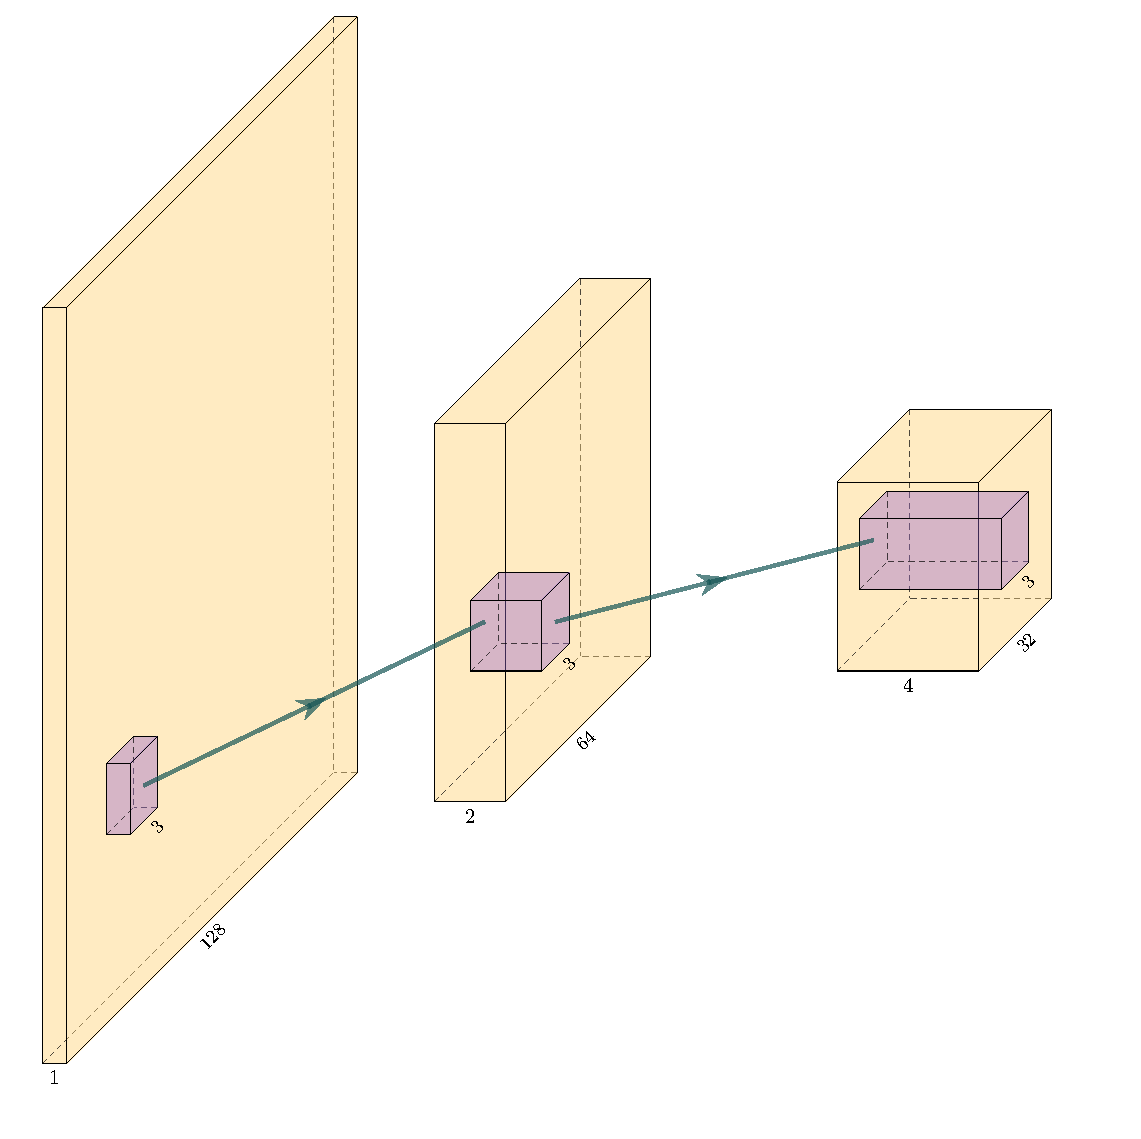
\includegraphics[width=\textwidth,height=5cm,keepaspectratio]{figures/cnn_schema.pdf}
    \caption{Schematic of a \ac{cnn} filter (purple) in the image data (orange) in 2D. The filter passes over the image, extracting a filtered representation of the input image. The image is downsampled spatially by striding or pooling. Convolutional filters are efficient due to weight sharing}
    \label{fig:cnn}
\end{figure}

For a two-dimensional \ac{cnn}, the convolution of the $m\times n$-dimensional image $G$ with a filter matrix $f$ can be expressed as:
\begin{equation}
G^{*}(x,y) = \sum_{i=1}^{n} \sum_{j=1}^{m} f(i,j)\cdot G(x-i+c,\; y-j+c),
\end{equation}
resulting in the central result $G^{*}$ around the coordinate $c$. Realistically, the calculation is done in the Fourier domain, due to the Convolution theorem reducing the computational complexity from $\mathcal{O}(n^2)$ to $\mathcal{O}(n \log n)$ with
\begin{equation}
    \mathcal{F}\{f * g\} = k\cdot \mathcal{F}\{f\}\cdot \mathcal{F}\{g\},
\end{equation}
with $\mathcal{F} \{ f\}$ denoting the Fourier transform of $f$ and $k$ being a normalization constant. This reduces the convolution to a simple multiplication in the Fourier domain, sped up by \ac{fft}.

\cref{fig:cnn} shows the schematic of connected convolutional layers in a \ac{cnn}. The network learns a specified number of $3\times3$ filters from the initial image. Strided convolutions with a step-size larger than 1 or Pooling layers are used to reduce the spatial extent of the image. The repeated downsampling of the image and extraction of convolutional filters has been shown to work for computer vision tasks. Historically, the CNN architecture AlexNet \citep{krizhevsky2012imagenet} was the first \ac{cnn} to enter the ImageNet challenge and improved the classification error rate from 25.8~\% to 16.4~\% (top-5 accuracy). This has propelled research in \acp{cnn}, resulting in error rates on ImageNet of 2.25~\% on top-5 accuracy in 2017 \citep{imagenetresults}.

\subsubsection{Generative Adversarial Networks}
\citet{Goodfellow2014-ax} introduced \acf{gan} as a combination of two \acp{cnn}. These \acfp{dcgan} exist in different modifications that draw from the original \ac{gan}, these modifications add more regularization and other feedback loops, as \acp{gan} are notoriously difficult to train without careful fine-tuning. These modifications include Wasserstein losses \citep{arjovsky2017wasserstein}, and gradient penalization \citep{gulrajani2017improved} for regularization, or cycle-consistent loss for unsupervised training \citep{zhu2017unpaired}.

\begin{figure}
    \centering
    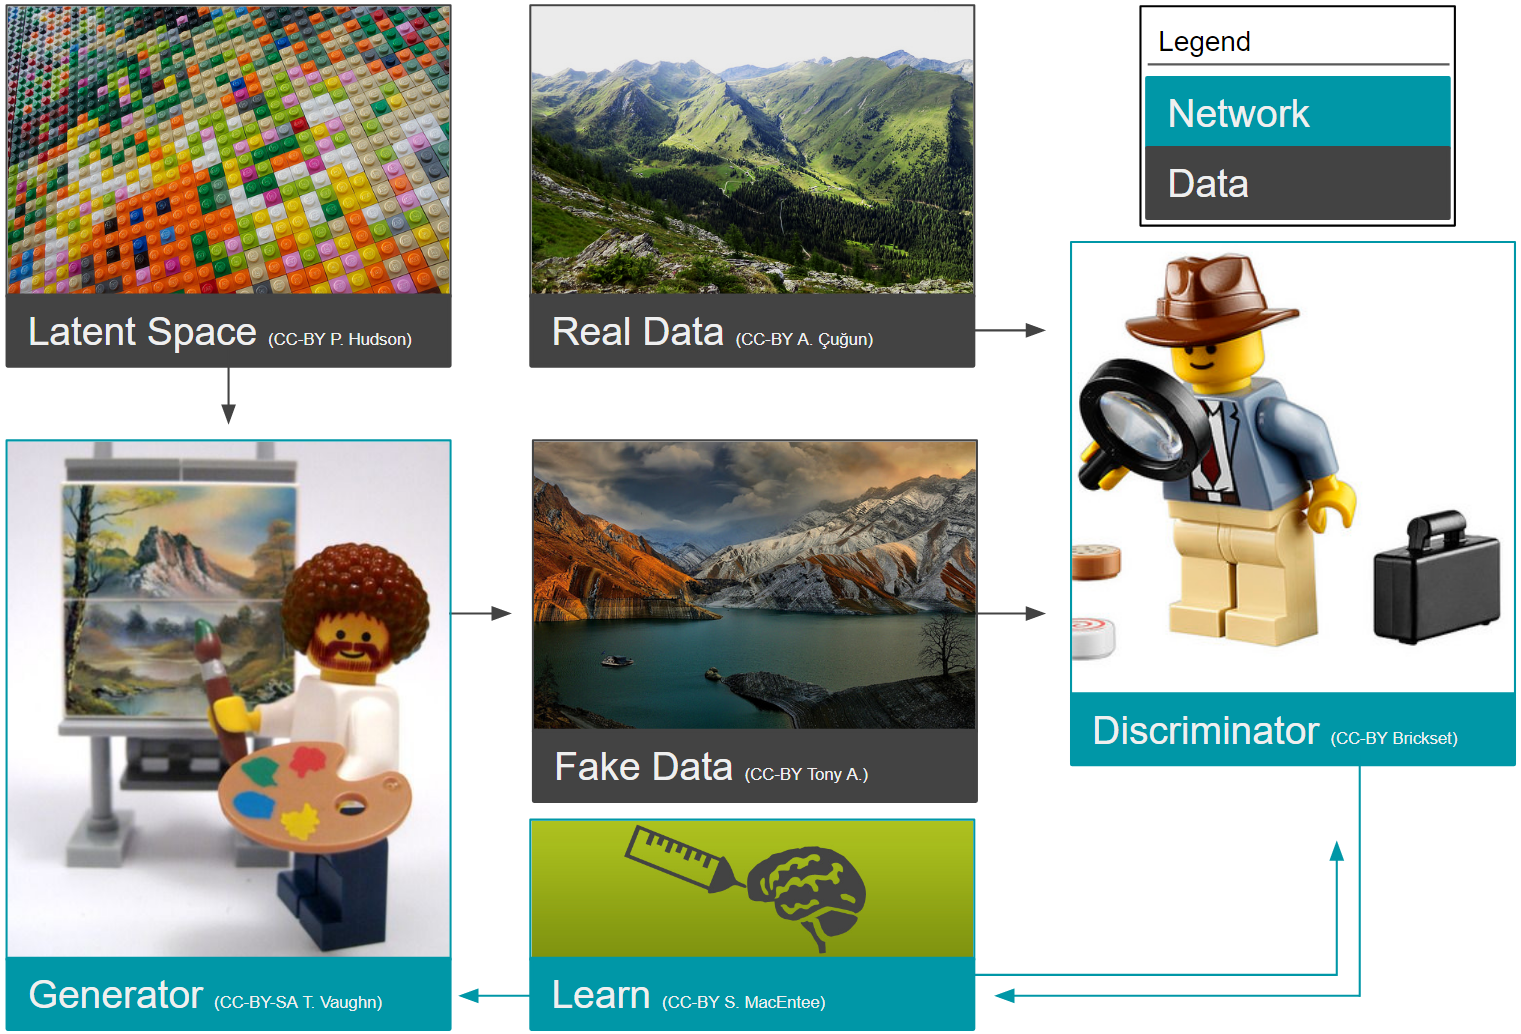
\includegraphics[width=\textwidth]{figures/GAN.PNG}
    \caption{Schematic of a \acl{gan}. The generator samples a latent space to generate fake data. The discriminator randomly obtains real or fake data and decides whether it was created by the generator or a real sample. The networks learn by gradient descent gaining information regardless of the discriminator being right}
    \label{fig:gan}
\end{figure}

\cref{fig:gan} shows the basic working of \acp{gan}. The arrows are colored in blue and grey, where the blue paths show network feedback and grey shows the progression of data. These networks learn from each other, where the generator draws from latent space (a noise vector) to create a fake version of a target. The discriminator tries to discern whether the presented data is real or generated from the adversarial generator. These networks leverage game theory to outperform each other and comparative networks. They reach a Nash equilibrium during training, which describes the concept on a non-cooperative game reaching steady state \citep{nash1951non}. 

% Considerations for Neural Architectures
\subsection{Neural Architectures}
\aclp{nn} can generally be assembled in different architectures. In \cref{fig:cnnsota} we present reported performances of neural architectures on the classification task of the ImageNet challenge. The colors in this figure express different classes of architectures. Early networks that broke ground as the new \aclp{sota} in image classification are the AlexNet, VGG-16, and VGG-19. These networks clearly do not leverage some tricks that modern CNNs implement, the VGG-16 with a relatively high amount of parameters is known to generalize well on transfer learning tasks however \citep{dramsch2018deep}. 

\begin{figure}
    \centering
    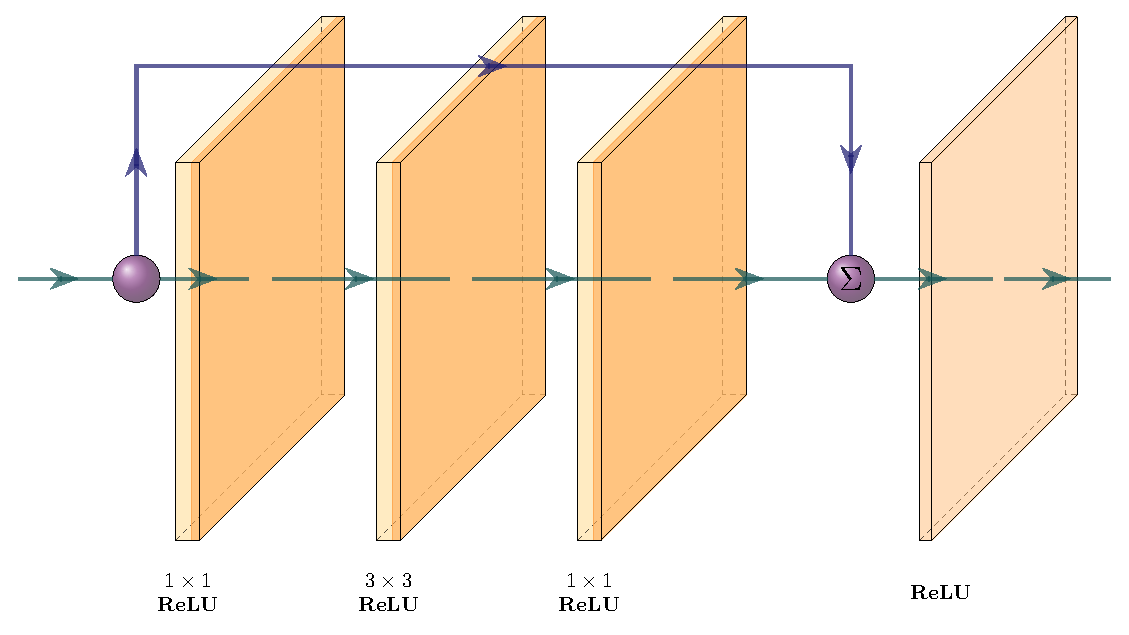
\includegraphics[width=\textwidth,height=5cm,keepaspectratio]{figures/resnet.pdf}
    \caption{Resnet Block with two $1\times1$ convolutional layers that frame a $3\times3$ convolutional layer with \ac{relu} activation each. The result being added with the original data, also known as identity.}
    \label{fig:resnet}
\end{figure}

Research into deep convolutional networks showed that the data in the network would lose signal with increasing depth. Hence, the limitation of VGG at 19 layers. Residual blocks introduced a solution to this problem by implementing a shortcut between the original data and the output from the block. \cref{fig:resnet} presents the original ResNet block architecture, which was used in ResNet-50 and ResNet-101 in \cref{fig:cnnsota} \citep{he2016deep}. Details on ResNet blocks differ, the main take-away being the sum or concatenation of the original data with the block output. DenseNets \citep{huang2017densely} and Inception-style networks \citep{szegedy2015going} are other approaches to build deeper \acp{nn}.

The categories of AmoebaNet, NASNet, and EfficientNet are a more recent development in neural architecture research, based on \acf{nas}. The AmoebaNet is based on Evolutionary Computing and hand-tuning the solution to search for an ideal neural architecture to solve the task \citep{real2019regularized}. The NASNet fixes the overall architecture, but uses a controler \ac{rnn} to modify the blocks within the architecture \citep{zoph2018learning}. The EfficientNet architecture was also acquired by \ac{nas}, by optimizing for both accuracy and FLOPS to reduce the computational cost \citep{tan2019efficientnet}. Moreover, \citet{tan2019efficientnet} derives a method of compound scaling for deep neural networks. While ResNet-50 and ResNet-101 differ only in depth, the authors derive a relationship between depth, width and resolution-scaling of deep neural networks.

\begin{figure}
    \centering
    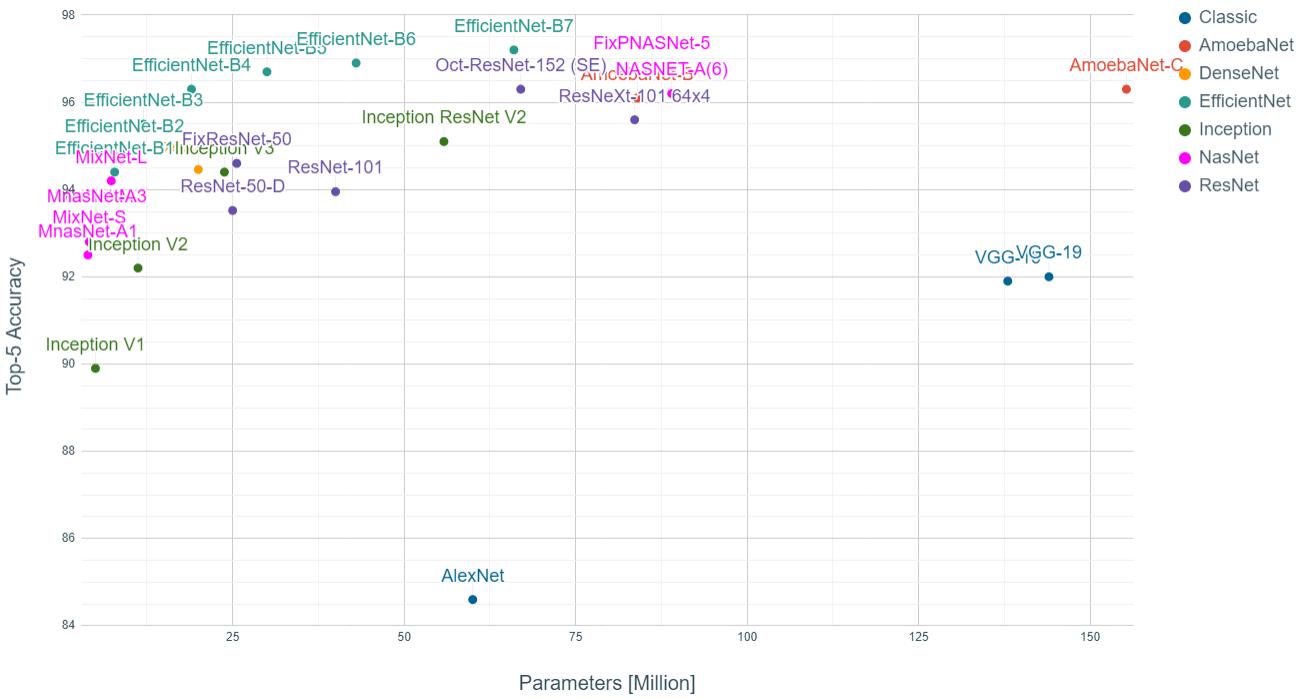
\includegraphics[width=1.1\textwidth]{figures/imagenetsota.png}
    \caption{Top-5 Accuracies of Neural Architectures on ImageNet plotted against Million Parameters, color-coded to similar network type. Data and references shown in \cref{tab:imagenet-sota}}
    \label{fig:cnnsota}
\end{figure}

Apart from building deeper networks for image classification, the neural architectures can serve as a  forcing function to the task the network is built for. Encoder-Decoder networks will compress the data with a combination of downsampling layers, which in the case of a computer vision could either be strided convolutions or pooling layers after convolutional layers. During these operations, the number of filters increases, while the spatial extent is diminished significantly. This encoding operation is equivalent to a lossy compression, with the low-dimensional layer called "code" or "bottleneck". The bottleneck is then upsampled by either strided transpose Convolutions or upsampling layers that perform a specified interpolation. This is the Decoder of the Encoder-Decoder pair. These networks can be used for data compresssion in \acp{ae}, where the decoder restores the original data as good as possible \citep{hinton2006reducing}. Alternatively, the Decoder can learn a dense classification task like semantic segmentation or seismic interpretation.

U-Nets present a special type of encoder-decoder networks, that learn semantic segmentation on from small datasets \citep{ronneberger2015unet}. They form a special kind of \ac{fcn} shown in \cref{fig:unet}. Originally developed on biomedical images, the network found wide acceptance in label sparse disciplines. The Unet implements shortcut connections between convolutional layers of equal extent in the Encoder and Decoder networks. This alleviates the pressure of the network learning and reconstructing the output data from the bottleneck in isolation. 

\begin{figure}
    \centering
    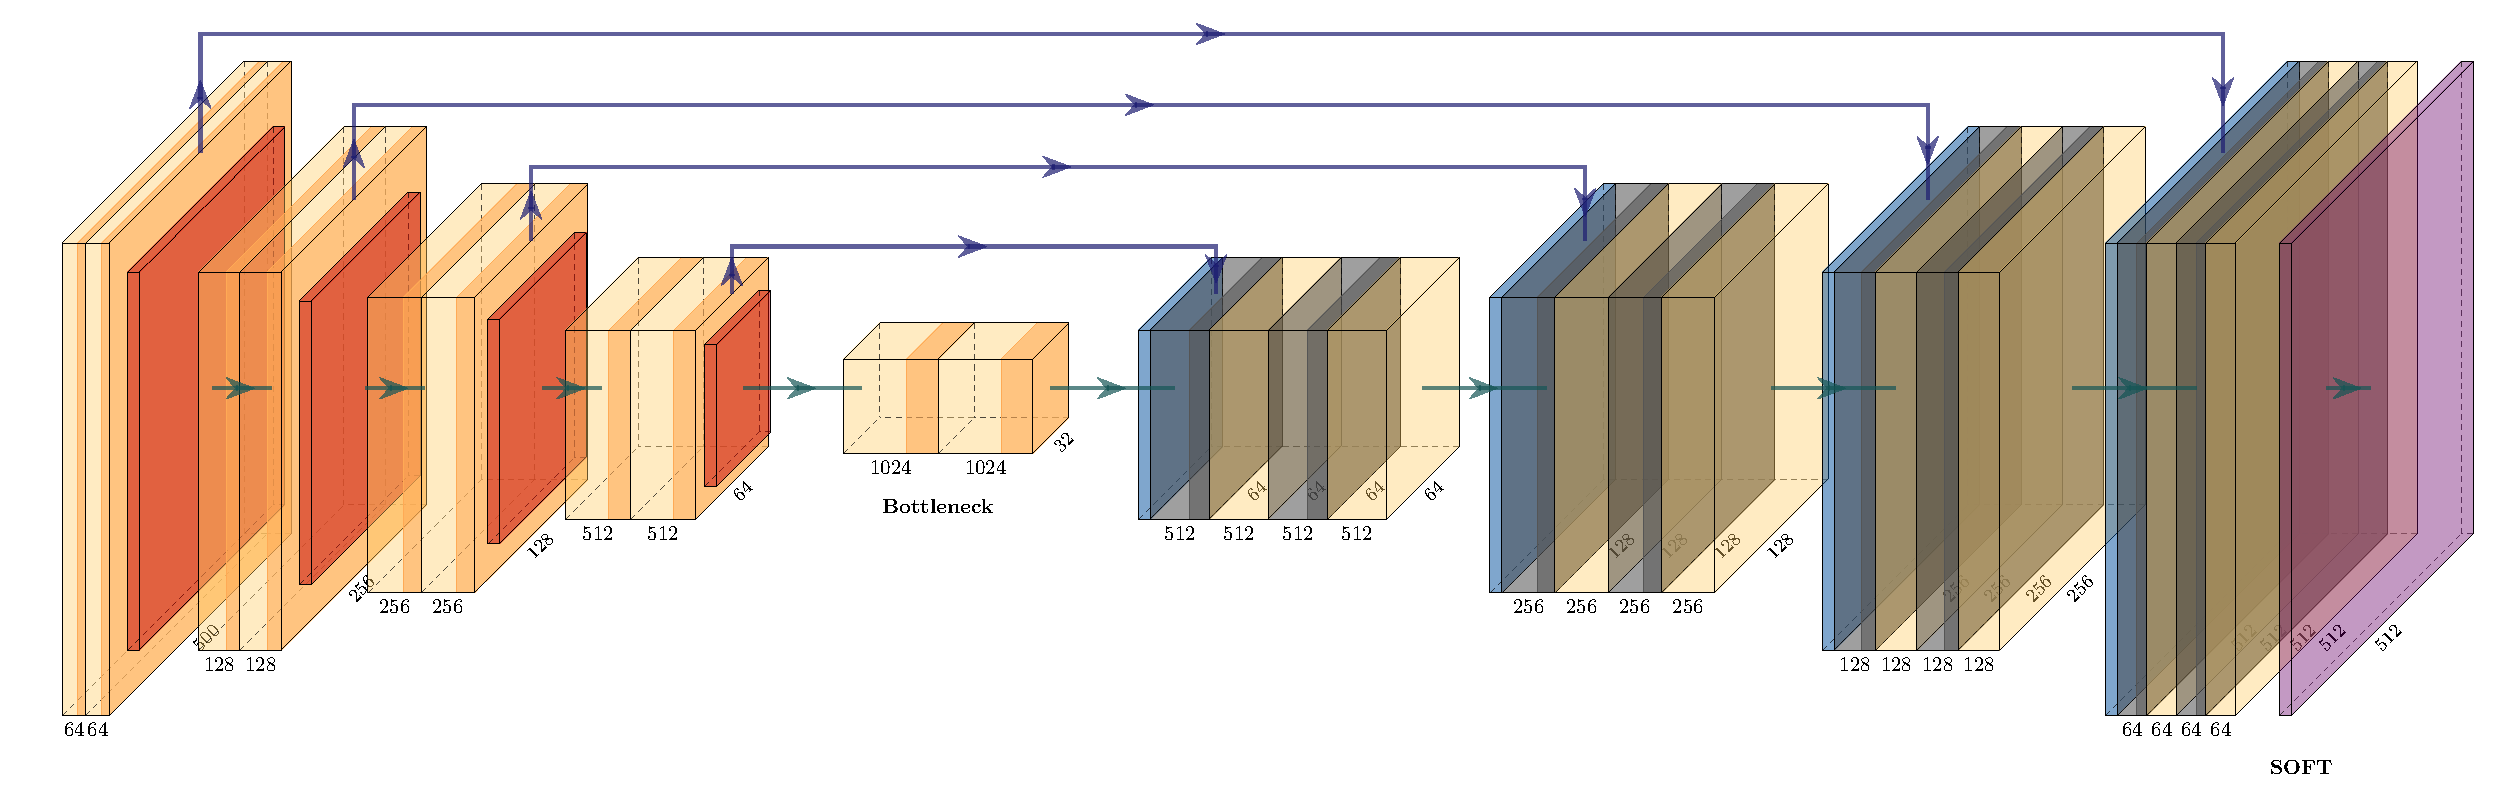
\includegraphics[width=\textwidth,height=5cm,keepaspectratio]{figures/unet.pdf}
    \caption{Unet after \citet{ronneberger2015unet} using 2D convolutional layers (yellow) with \ac{relu} activation (orange) and skip connection between equal-dimensional layers. The Encoder uses pooling (red), while the Decoder uses Upsampling layers (blue), witha final SoftMax layer (purple) for classification / semantic segmentation}
    \label{fig:unet}
\end{figure}